\documentclass{article}

\usepackage[]{../.template/xrcise}

\subject{Natural Language Processsing}
\semester{Winter 2024}
\author{Leopold Lemmermann}

\begin{document}\createtitle

\sheet{Lecture questions}

\begin{exercise}{Web as an application area for NLP}
  The web is an application area for NLP. Provide examples of applications.

  \begin{solution}
    Examples include:
    \begin{itemize}
        \item Internet of Services
        \item Community mining
        \item Information retrieval
        \item Machine translation for web-based content
    \end{itemize}
  \end{solution}
\end{exercise}

\begin{exercise}{Web as a resource for NLP}
  How can the web improve the quality of NLP? Provide examples.

  \begin{solution}
    Examples include:
    \begin{itemize}
        \item Web as Corpus
        \item Analyzing web-based knowledge repositories
        \item Extracting structured information from unstructured web data
        \item Using web-scale data for training language models
    \end{itemize}
  \end{solution}
\end{exercise}

\begin{exercise}{Morphological analysis}
  Identify all stems and affixes (prefix, suffix, infix, circumfix) in the following words: "index," "incorrect," "interesting."

  \begin{solution}
    Morphological breakdown:
    \begin{itemize}
        \item \textbf{index}: stem = "index"
        \item \textbf{incorrect}: prefix = "in," stem = "correct"
        \item \textbf{interesting}: stem = "interest," suffix = "ing"
    \end{itemize}
  \end{solution}
\end{exercise}

\begin{exercise}{Stemming vs lemmatization}
  In contrast to lemmatization, stemming does not necessarily return a valid word form. Why is stemming still useful?

  \begin{solution}
    Stemming is still useful because:
    \begin{itemize}
        \item It is faster and computationally less expensive.
        \item It simplifies implementation for applications like Information Retrieval.
        \item It can still group similar words under a common base, which is often sufficient.
    \end{itemize}
  \end{solution}
\end{exercise}

\begin{exercise}{Corpus definition and usage}
  What is a corpus, and how can it be built and used for linguistic analysis?

  \begin{solution}
    \begin{itemize}
        \item \textbf{Corpus definition}: A corpus is a large and structured set of texts, often used for linguistic research.
        \item \textbf{How to build}: Collect text data, preprocess it (cleaning, normalization), and annotate it for specific tasks.
        \item \textbf{Usage}: Analyze linguistic patterns, train NLP models, and evaluate machine learning algorithms.
    \end{itemize}
  \end{solution}
\end{exercise}

\begin{exercise}{NLP datasets}
  What are NLP datasets, and why are they important?

  \begin{solution}
    \begin{itemize}
        \item \textbf{Definition}: NLP datasets are collections of annotated or unannotated text data designed for specific NLP tasks (e.g., sentiment analysis, translation).
        \item \textbf{Importance}:
        \begin{itemize}
            \item Serve as a foundation for training and testing machine learning models.
            \item Enable reproducibility in research.
            \item Facilitate comparisons between models and techniques.
        \end{itemize}
    \end{itemize}
  \end{solution}
\end{exercise}

\begin{exercise}{Corpus and dataset annotation}
  What is the annotation process for a corpus or dataset, and how does it impact machine learning applications?

  \begin{solution}
    \begin{itemize}
        \item \textbf{Annotation process}: Adding labels or metadata to text data (e.g., part-of-speech tags, sentiment labels, named entities).
        \item \textbf{Impact on machine learning}:
        \begin{itemize}
            \item Improves model performance by providing high-quality training data.
            \item Enables supervised learning by associating input with output labels.
            \item Impacts scalability and generalization of models depending on annotation quality.
        \end{itemize}
    \end{itemize}
  \end{solution}
\end{exercise}

\begin{exercise}{Large-scale dataset collection using crowdsourcing}
  What are the main strategies for large-scale dataset collection using crowdsourcing?

  \begin{solution}
    Strategies include:
    \begin{itemize}
        \item \textbf{Task design}: Clearly define annotation tasks with examples and guidelines.
        \item \textbf{Platform selection}: Use platforms like Amazon Mechanical Turk or Prolific.
        \item \textbf{Quality control}: Use redundancy (multiple annotators per task) and include test questions to ensure reliability.
        \item \textbf{Data aggregation}: Combine annotations using majority voting or statistical models.
    \end{itemize}
  \end{solution}
\end{exercise}

% Q: Why are more features not always better for learning a
% classifier?
% A: More training data might be needed; Dependent features
% might lead to deficient models; Some ML algorithms can only deal
% with specific data types; Slower.
% Q: What is the typical type of input data that a sequence tagger
% training step requires?
% A: Labeled training text. (e.g. POS, NER)



\setcounter{section}{2022}
\sheet{1st exam}

\begin{exercise}{Tokenization}
  Give at least 3 examples of ambiguity in tokenization.

  \begin{solution}
    \begin{enumerate}
        \item \textbf{Hyphenated words}: Does "state-of-the-art" count as one token or three?
        \item \textbf{Contractions}: Should "don't" be treated as one token or split into "do" and "n't"?
        \item \textbf{Punctuation}: How should punctuation like periods in "U.S." or apostrophes in possessives ("John's book") be handled?
    \end{enumerate}
  \end{solution}
\end{exercise}

\begin{exercise}{Parse trees}
  "\textit{John shot the man with the gun}". Draw all possible parse trees for this sentence using the English grammar. What types of syntactic ambiguity are present?

  \begin{solution}
    A parse tree can be drawn using the following structures: $S, N, V, Det, P, NP, VP, PP$. This is an example of attachment ambiguity. The prepositional phrase "with the gun" can attach to either "shot" or "the man".
  \end{solution}
\end{exercise}

\begin{exercise}{Stemming and lemmatization}
  What is the difference between stemming and lemmatization?

  \begin{solution}
    While stemming reduces a word to its base form by removing pre- and suffices ("running" → "run"), lemmatization considers the word's context and grammar to find its dictionary form ("better" → "good"). Lemmatization is more precise than stemming but computationally more expensive.
  \end{solution}
\end{exercise}

\begin{exercise}{Web as corpus}
  List 4 issues you have to deal with when using the web as a corpus for NLP purposes and explain each.

  \begin{solution}
    \begin{enumerate}
        \item \textbf{Noise}: Content may contain errors, irrelevant information, or non-standard grammar.
        \item \textbf{Duplicates}: Identical or nearly identical data appears multiple times.
        \item \textbf{Bias}: Web content often reflects societal biases, which can skew analyses.
        \item \textbf{Reproducability}: Web pages change frequently, making reproducibility challenging.
    \end{enumerate}
  \end{solution}
\end{exercise}

\begin{exercise}{Cross-language QA}
  How does cross-language QA work and what are the main issues?

  \begin{solution}
    Cross-language QA involves answering questions in one language based on information in another. This is accomplished by translating the question, retrieving relevant information in the target language, and generating an answer. Challenges include translation errors, cultural differences.
  \end{solution}
\end{exercise}

\begin{exercise}{Machine learning pipeline}
  What are the main concepts in a machine learning pipeline?

  \begin{solution}
    Data Preprocessing $\to$ Feature extraction $\to$ Model training $\to$ Evaluation $\to$ Deployment
  \end{solution}
\end{exercise}

\begin{exercise}{IR evaluation}
  What are the problems with precision, recall, and F-measure in IR? How can these be improved? Why is Cohen's Kappa better?

  \begin{solution}
    \begin{itemize}
        \item \textbf{Precision}: How relevant are the retrieved documents? Favors retrieving fewer documents.
        \item \textbf{Recall}: How many of the relevant documents were retrieved? Favors retrieving more documents.
        \item \textbf{F-measure}: Harmonic mean of precision and recall. Balances the two metrics but not adjustable.
        \item \textbf{Cohen's Kappa}: Measures inter-annotator agreement, accounting for chance agreement. Better for evaluating IR systems because it considers agreement beyond chance.
    \end{itemize}
  \end{solution}
\end{exercise}

\begin{exercise}{IR evaluation}
  Calculate P@5, P@10, and MAP for the given IR ranked result list. Analyze both IR system A and system B.

  \begin{solution}
    For P@5, P@10, and MAP:
    \begin{itemize}
        \item \textbf{P@5}: Count relevant documents in the top 5 results and divide by 5.
        \item \textbf{P@10}: Same calculation for the top 10 results.
        \item \textbf{MAP}: Average Precision for each query, then average across all queries.
    \end{itemize}
    Steps:
    \begin{itemize}
        \item Identify positions of relevant documents in ranked lists.
        \item Calculate precision at each relevant position.
        \item Take mean of these precision values.
    \end{itemize}
  \end{solution}
\end{exercise}

\begin{exercise}{Naive Bayes and SVM}
  Which of the following statements are correct?
  \begin{enumerate}
    \item Features for Naive Bayes classifiers do not need to be uncorrelated.
    \item Naive Bayes is slow to train.
    \item SVM itself is a multi-label classifier.
    \item SVM handles sparse data well.
  \end{enumerate}

  \begin{solution}
    Correct statements:
    \begin{enumerate}
        \item \textbf{True}: Features for Naive Bayes do not need to be uncorrelated, though it assumes independence for computation.
        \item \textbf{False}: Naive Bayes is fast to train, not slow.
        \item \textbf{False}: SVM is not inherently multi-label but can be adapted for multi-label classification.
        \item \textbf{True}: SVM handles sparse data well due to its kernel functions.
    \end{enumerate}
  \end{solution}
\end{exercise}

\begin{exercise}{Corpus construction}
  How can a corpus be constructed for linguistic purposes from web data, and how can it be made usable?

  \begin{solution}
    Steps for constructing a corpus:
    \begin{enumerate}
        \item \textbf{Data collection}: Crawl web pages, scrape data, or gather domain-specific text.
        \item \textbf{Cleaning}: Remove duplicates, irrelevant content, and normalize text.
        \item \textbf{Annotation}: Add metadata or labels for tasks like classification or parsing.
        \item \textbf{Usability}: Store in accessible formats (e.g., JSON, XML) and document the corpus for ease of use.
    \end{enumerate}
  \end{solution}
\end{exercise}

\begin{exercise}{Pragmatics and discourse analysis}
  Why are pragmatics and discourse analysis difficult?

  \begin{solution}
    Challenges in pragmatics and discourse analysis:
    \begin{itemize}
        \item \textbf{Context dependency}: Understanding depends heavily on prior sentences or external knowledge.
        \item \textbf{Ambiguity}: Words and phrases can have multiple meanings depending on the situation.
        \item \textbf{Social norms}: Interpretations vary based on cultural or societal factors.
    \end{itemize}
  \end{solution}
\end{exercise}

\begin{exercise}{Hate speech}
  Define hate speech and explain how to construct a hate speech classifier.

  \begin{solution}
    \begin{itemize}
        \item \textbf{Definition}: Hate speech involves language that attacks or discriminates against individuals or groups based on attributes like race, religion, ethnicity, gender, or sexual orientation.
        \item \textbf{Constructing a hate speech classifier}:
        \begin{enumerate}
            \item Collect labeled datasets with examples of hate speech and non-hate speech.
            \item Preprocess text (e.g., tokenization, removing stop words).
            \item Extract features (e.g., bag-of-words, TF-IDF, embeddings).
            \item Train a supervised machine learning model (e.g., Naive Bayes, SVM, or deep learning models like LSTMs or transformers).
            \item Evaluate the classifier using metrics like precision, recall, and F1-score.
        \end{enumerate}
    \end{itemize}
  \end{solution}
\end{exercise}

\begin{exercise}{Counter hate speech}
  What is counter hate speech, and how can a system be constructed for it?

  \begin{solution}
    \begin{itemize}
        \item \textbf{Definition}: Counter hate speech is content designed to reduce the impact of hate speech, often by promoting positive, empathetic, or factual responses.
        \item \textbf{Constructing a counter hate speech system}:
        \begin{enumerate}
            \item Collect datasets of effective counter hate responses.
            \item Train models to generate or retrieve appropriate responses based on the hate speech content.
            \item Use sentiment analysis and empathy detection to craft responses.
            \item Deploy the system in platforms like social media or forums, ensuring ethical considerations are addressed.
        \end{enumerate}
    \end{itemize}
  \end{solution}
\end{exercise}

\begin{exercise}{Crowdsourced annotation}
  What is the workflow for crowdsourced annotation?

  \begin{solution}
    Steps in a crowdsourced annotation workflow:
    \begin{enumerate}
        \item \textbf{Task design}: Define the annotation task clearly with examples and instructions.
        \item \textbf{Platform setup}: Use a crowdsourcing platform (e.g., Amazon Mechanical Turk, Prolific).
        \item \textbf{Quality control}: Include test questions and redundancy (multiple annotators per item) to ensure data reliability.
        \item \textbf{Data aggregation}: Aggregate annotations using majority voting or weighted schemes.
        \item \textbf{Evaluation}: Analyze annotation quality and address inconsistencies.
    \end{enumerate}
  \end{solution}
\end{exercise}

\begin{exercise}{Web corpus}
  Why do duplicates exist on the web, and how can they be detected?

  \begin{solution}
    \begin{itemize}
        \item \textbf{Duplicates}: Duplicates arise from mirrored websites, copied content, or redundant crawls.
        \item \textbf{Detection methods}:
        \begin{itemize}
            \item Hashing (e.g., MD5 or SHA): Compare hash values of documents.
            \item Similarity measures: Use cosine similarity or Jaccard index on n-grams.
            \item Structural analysis: Detect similarity in HTML structure.
        \end{itemize}
    \end{itemize}
  \end{solution}
\end{exercise}

\begin{exercise}{QA vs IR}
  What are the differences between Question Answering (QA) and Information Retrieval (IR)?

  \begin{solution}
    Differences between QA (Question Answering) and IR (Information Retrieval):
    \begin{itemize}
        \item \textbf{Goal}:
        \begin{itemize}
            \item QA aims to provide direct answers.
            \item IR retrieves documents containing relevant information.
        \end{itemize}
        \item \textbf{Processing}:
        \begin{itemize}
            \item QA requires deeper natural language understanding.
            \item IR focuses on keyword matching and ranking.
        \end{itemize}
        \item \textbf{Applications}:
        \begin{itemize}
            \item QA: Chatbots, customer support.
            \item IR: Search engines.
        \end{itemize}
    \end{itemize}
  \end{solution}
\end{exercise}

\begin{exercise}{Cross-language QA}
  What are the applications of multi-language QA, and what difficulties arise?

  \begin{solution}
    \begin{itemize}
        \item \textbf{Applications}: Multi-language QA systems are used in global customer support, cross-border e-commerce, and multi-language search engines.
        \item \textbf{Difficulties}:
        \begin{itemize}
            \item Translation errors can distort queries or results.
            \item Cultural and linguistic differences complicate understanding and generating answers.
            \item Lack of high-quality bilingual corpora for training.
        \end{itemize}
    \end{itemize}
  \end{solution}
\end{exercise}

\begin{exercise}{Language detection}
  How does language detection work?

  \begin{solution}
    Approaches for language detection:
    \begin{enumerate}
        \item \textbf{N-gram analysis}: Compare n-grams of text against language-specific frequency profiles.
        \item \textbf{Machine learning models}: Use classifiers trained on labeled text for different languages.
        \item \textbf{Lexicon-based methods}: Match words in the text to dictionaries of different languages.
        \item \textbf{Hybrid approaches}: Combine multiple methods for higher accuracy.
    \end{enumerate}
  \end{solution}
\end{exercise}

\begin{exercise}{Factual QA vs opinionated QA}
  What are the differences between factual QA and opinionated QA, and which is easier to evaluate?

  \begin{solution}
    \begin{itemize}
        \item \textbf{Factual QA}: Deals with objective information (e.g., "What is the capital of France?").
        \item \textbf{Opinionated QA}: Involves subjective answers (e.g., "Is Paris a good travel destination?").
        \item \textbf{Evaluation}: Factual QA is easier to evaluate as answers can be verified against ground truth. Opinionated QA requires subjective or aggregated assessments.
    \end{itemize}
  \end{solution}
\end{exercise}

\begin{exercise}{RAG and LangChain}
  What is Retrieval-Augmented Generation (RAG), and how does LangChain assist in implementing it?

  \begin{solution}
    \begin{itemize}
        \item \textbf{RAG (Retrieval-Augmented Generation)}: Combines retrieval models with generative models to produce context-aware answers. External knowledge is retrieved and fed into the generation model.
        \item \textbf{LangChain}: A framework for building applications with large language models, offering tools for integrating RAG systems. It manages chaining retrieval and generation steps efficiently.
    \end{itemize}
  \end{solution}
\end{exercise}

\begin{exercise}{Sentiment analysis}
  Compare sentiment analysis using supervised approaches and lexicon-based approaches.

  \begin{solution}
    \begin{itemize}
        \item \textbf{Supervised learning}: Uses labeled data to train machine learning models.
        \begin{itemize}
            \item \textbf{Advantages}: High accuracy with large datasets.
            \item \textbf{Drawbacks}: Relies on annotated data and is domain-dependent.
        \end{itemize}
        \item \textbf{Lexicon-based approaches}: Use sentiment dictionaries to determine polarity.
        \begin{itemize}
            \item \textbf{Advantages}: Simplicity and no training requirement.
            \item \textbf{Drawbacks}: Limited contextual understanding and poor performance on complex text.
        \end{itemize}
    \end{itemize}
  \end{solution}
\end{exercise}

\begin{exercise}{Edit distance}
  Calculate the Minimum Edit Distance for "TAC" vs. "CAT" and list all possible word outcomes.

  \begin{solution}
    \begin{itemize}
        \item \textbf{Minimum Edit Distance for "TAC" and "CAT"}:
        \[
        \begin{array}{c|c|c|c|c}
            &  & C & A & T \\
            \hline
            & 0 & 1 & 2 & 3 \\
            T & 1 & 1 & 2 & 2 \\
            A & 2 & 2 & 1 & 2 \\
            C & 3 & 2 & 2 & 2 \\
        \end{array}
        \]
        \item \textbf{Word outcomes}: Possible outcomes from edits:
        \begin{enumerate}
            \item CAT
            \item TAT
            \item TAC
            \item CAC
        \end{enumerate}
    \end{itemize}
  \end{solution}
\end{exercise}



\setcounter{section}{2021}
\sheet{1st exam}

\begin{exercise}{Corpus construction}
  How would you construct a corpus for linguistic purposes and how can it be made usable?

  \begin{solution}
    \begin{enumerate}
        \item \textbf{Data collection}: Gather data from relevant sources (e.g., web crawling, domain-specific text).
        \item \textbf{Cleaning and preprocessing}: Remove duplicates, non-linguistic content, and normalize text (e.g., case normalization, tokenization).
        \item \textbf{Annotation}: Add metadata or linguistic labels (e.g., POS tags, syntactic trees) to the text.
        \item \textbf{Storage}: Store the corpus in an accessible format like JSON, XML, or relational databases.
        \item \textbf{Documentation}: Provide guidelines and metadata about the corpus for user understanding.
    \end{enumerate}
  \end{solution}
\end{exercise}

\begin{exercise}{Pragmatics and discourse analysis}
  Why are pragmatics and discourse analysis difficult?

  \begin{solution}
    \begin{itemize}
        \item \textbf{Context dependency}: Requires understanding of the broader context beyond sentence boundaries.
        \item \textbf{Ambiguity}: Words or phrases can have multiple meanings depending on the discourse.
        \item \textbf{Cultural and social norms}: Interpretation is influenced by societal and cultural factors.
        \item \textbf{Incomplete information}: Missing parts of conversations or text make it harder to analyze.
    \end{itemize}
  \end{solution}
\end{exercise}

\begin{exercise}{Sequence tagging and CRF}
  Define sequence tagging and explain what a Conditional Random Field (CRF) is.

  \begin{solution}
    \begin{itemize}
        \item \textbf{Sequence tagging}: The process of assigning labels to each element in a sequence (e.g., part-of-speech tagging, named entity recognition).
        \item \textbf{Conditional Random Field (CRF)}: A probabilistic model used for structured prediction in sequence data. It considers the context of neighboring labels to improve accuracy.
    \end{itemize}
  \end{solution}
\end{exercise}

\begin{exercise}{Minimum edit distance}
  Calculate the Minimum Edit Distance for "TAC" vs. "CAT" (a table is given). List all possible outcomes.

  \begin{solution}
    \begin{itemize}
        \item \textbf{Minimum Edit Distance Table}:
        \[
        \begin{array}{c|c|c|c|c}
            &  & C & A & T \\
            \hline
            & 0 & 1 & 2 & 3 \\
            T & 1 & 1 & 2 & 2 \\
            A & 2 & 2 & 1 & 2 \\
            C & 3 & 2 & 2 & 2 \\
        \end{array}
        \]
        \item \textbf{Outcomes}:
        \begin{enumerate}
            \item CAT
            \item TAT
            \item TAC
            \item CAC
        \end{enumerate}
    \end{itemize}
  \end{solution}
\end{exercise}

\begin{exercise}{IR evaluation}
  Calculate P@5 and MAP for given ranked IR results for two systems.

  \begin{solution}
    \begin{itemize}
        \item \textbf{P@5}: Count relevant documents in the top 5 results and divide by 5.
        \item \textbf{MAP}: For each query, calculate average precision across relevant documents and average these scores.
    \end{itemize}
  \end{solution}
\end{exercise}

\begin{exercise}{Hate speech}
  Define hate speech and how to construct a hate speech classifier.

  \begin{solution}
    \begin{itemize}
        \item \textbf{Definition}: Hate speech targets individuals or groups based on attributes like race, religion, gender, or orientation.
        \item \textbf{Classifier construction}:
        \begin{enumerate}
            \item Collect labeled datasets of hate and non-hate speech.
            \item Preprocess data by removing noise and tokenizing.
            \item Train a machine learning model (e.g., Naive Bayes, SVM, transformers).
            \item Evaluate using metrics like F1-score, precision, and recall.
        \end{enumerate}
    \end{itemize}
  \end{solution}
\end{exercise}

\begin{exercise}{Counter hate speech}
  What is counter hate speech, and how can a system be constructed for it?

  \begin{solution}
    \begin{itemize}
        \item \textbf{Definition}: Counter hate speech neutralizes hate content by promoting positive or factual responses.
        \item \textbf{System construction}:
        \begin{enumerate}
            \item Collect examples of effective counter hate responses.
            \item Use NLP techniques to classify hate speech and generate counter-responses.
            \item Train models on empathy and sentiment analysis for response generation.
        \end{enumerate}
    \end{itemize}
  \end{solution}
\end{exercise}

\begin{exercise}{Sentiment lexicon extension}
  How can sentiment analysis be improved using lexicon extensions from distributed thesauruses?

  \begin{solution}
    \begin{itemize}
        \item \textbf{Lexicon extension}: Expand sentiment dictionaries using related terms from distributed word embeddings like Word2Vec or GloVe.
        \item \textbf{Process}:
        \begin{enumerate}
            \item Identify synonyms, antonyms, or similar words in embedding spaces.
            \item Update lexicons with these terms to improve coverage.
            \item Validate new terms to ensure sentiment accuracy.
        \end{enumerate}
    \end{itemize}
  \end{solution}
\end{exercise}
\begin{exercise}{Sentiment analysis}
  Discuss sentiment detection using lexicon based vs. supervised learning approaches.

  \begin{solution}
    \begin{itemize}
        \item \textbf{Lexicon-based approaches}: 
        \begin{itemize}
            \item Use pre-built dictionaries of words with sentiment labels (e.g., positive, negative).
            \item Advantages:
                \begin{itemize}
                    \item Easy to implement and interpret.
                    \item No need for labeled training data.
                \end{itemize}
            \item Disadvantages:
                \begin{itemize}
                    \item Limited to the coverage of the lexicon.
                    \item Poor performance on context-dependent sentiment (e.g., sarcasm).
                \end{itemize}
        \end{itemize}
        \item \textbf{Supervised learning approaches}:
        \begin{itemize}
            \item Train machine learning models on labeled data to classify sentiment.
            \item Advantages:
                \begin{itemize}
                    \item Can learn from context and handle subtle sentiment expressions.
                    \item Scalable to large datasets.
                \end{itemize}
            \item Disadvantages:
                \begin{itemize}
                    \item Requires annotated data, which can be costly to obtain.
                    \item More computationally intensive than lexicon-based approaches.
                \end{itemize}
        \end{itemize}
    \end{itemize}
  \end{solution}
\end{exercise}

\begin{exercise}{Sentiment analysis}
  Why is lexicon based sentiment analysis not enough?

  \begin{solution}
    \begin{itemize}
        \item \textbf{Context-dependence}: Lexicons fail to account for how sentiment changes with context.
        \item \textbf{Negation handling}: Sentences like "not bad" may be incorrectly classified without understanding negation.
        \item \textbf{Ambiguity}: Words can have different sentiments in different contexts (e.g., "hot" in weather vs. arguments).
        \item \textbf{Domain-specific issues}: Lexicons often do not cover domain-specific terms or slang.
    \end{itemize}
  \end{solution}
\end{exercise}

\begin{exercise}{Naive Bayes and SVM}
  Which of the following 4 are correct:
  \begin{enumerate}
    \item Features for Naive Bayes classifiers do not need to be uncorrelated.
    \item Naive Bayes is slow to train.
    \item SVM itself is a multi-label classifier.
    \item SVM handles sparse data well.
  \end{enumerate}

  \begin{solution}
    \begin{itemize}
        \item \textbf{Correct}: 
        \begin{itemize}
            \item Features for Naive Bayes classifiers do not need to be uncorrelated.
            \item SVM handles sparse data well.
        \end{itemize}
        \item \textbf{Incorrect}:
        \begin{itemize}
            \item Naive Bayes is actually fast to train.
            \item SVM is not inherently multi-label but can be adapted for multi-label classification.
        \end{itemize}
    \end{itemize}
  \end{solution}
\end{exercise}

\begin{exercise}{Language detection}
  Explain approaches for language detection.

  \begin{solution}
    \begin{itemize}
        \item \textbf{N-gram analysis}: Compare the frequency of character n-grams against language-specific profiles.
        \item \textbf{Machine learning models}: Train classifiers (e.g., SVM, neural networks) using labeled text data for various languages.
        \item \textbf{Lexicon-based methods}: Use dictionaries to match input text to language-specific words.
        \item \textbf{Hybrid approaches}: Combine n-gram, lexicon, and machine learning techniques for better accuracy.
    \end{itemize}
  \end{solution}
\end{exercise}

\begin{exercise}{Crowdsourced annotation}
  Explain the crowdsourced annotation workflow.

  \begin{solution}
    Steps in a crowdsourced annotation workflow:
    \begin{enumerate}
        \item \textbf{Task design}: Define the annotation task with clear instructions and examples.
        \item \textbf{Platform setup}: Deploy the task on crowdsourcing platforms like Amazon Mechanical Turk.
        \item \textbf{Quality control}: Use redundancy by assigning multiple annotators to the same task and include test questions.
        \item \textbf{Data aggregation}: Combine annotations using majority voting or weighted scoring methods.
        \item \textbf{Evaluation}: Analyze the consistency and reliability of annotations.
    \end{enumerate}
  \end{solution}
\end{exercise}

\begin{exercise}{Tokenization ambiguities}
  What are the ambiguities for tokenization?

  \begin{solution}
    Ambiguities in tokenization include:
    \begin{itemize}
        \item \textbf{Hyphenation}: Is "state-of-the-art" one token or three?
        \item \textbf{Punctuation}: Should periods in abbreviations (e.g., "U.S.") be separated?
        \item \textbf{Contractions}: Should "don't" be split into "do" and "n't"?
        \item \textbf{Language differences}: Tokenization rules vary by language (e.g., Chinese characters vs. English words).
    \end{itemize}
  \end{solution}
\end{exercise}

\begin{exercise}{QA vs IR}
  What are the differences between QA and IR?

  \begin{solution}
    Differences between QA and IR:
    \begin{itemize}
        \item \textbf{Goal}:
        \begin{itemize}
            \item QA provides direct answers to user queries.
            \item IR retrieves documents that may contain relevant information.
        \end{itemize}
        \item \textbf{Processing}:
        \begin{itemize}
            \item QA requires natural language understanding and reasoning.
            \item IR focuses on keyword matching and ranking algorithms.
        \end{itemize}
        \item \textbf{Applications}:
        \begin{itemize}
            \item QA is used in chatbots and virtual assistants.
            \item IR powers search engines like Google.
        \end{itemize}
    \end{itemize}
  \end{solution}
\end{exercise}

\begin{exercise}{Cross-language QA}
  What are the challenges in cross-language QA?

  \begin{solution}
    Challenges in cross-language QA include:
    \begin{itemize}
        \item \textbf{Translation errors}: Inaccurate translations can distort queries or answers.
        \item \textbf{Lack of parallel resources}: Few high-quality bilingual corpora exist for certain language pairs.
        \item \textbf{Cultural differences}: Questions or answers may need cultural adaptation.
        \item \textbf{Mismatched structures}: Linguistic differences make aligning queries and answers difficult.
    \end{itemize}
  \end{solution}
\end{exercise}

\begin{exercise}{Stemming vs lemmatization}
  What is the difference between stemming and lemmatization?

  \begin{solution}
    \begin{itemize}
        \item \textbf{Stemming}: Reduces a word to its root by chopping off affixes (e.g., "running" → "run"). It is less precise and may produce non-words.
        \item \textbf{Lemmatization}: Converts a word to its base form (lemma) based on its context (e.g., "better" → "good"). It is more accurate but computationally expensive.
    \end{itemize}
  \end{solution}
\end{exercise}

\begin{exercise}{Web corpus}
  Why are duplicates on the web, and how can they be detected?

  \begin{solution}
    \begin{itemize}
        \item \textbf{Reasons for duplicates}:
        \begin{itemize}
            \item Content mirroring across websites.
            \item Republishing of syndicated articles.
            \item Crawling the same site multiple times.
        \end{itemize}
        \item \textbf{Detection methods}:
        \begin{itemize}
            \item Hashing (e.g., MD5, SHA) to compare file contents.
            \item Cosine similarity or Jaccard index for text comparisons.
            \item Comparing HTML structure or metadata.
        \end{itemize}
    \end{itemize}
  \end{solution}
\end{exercise}

\begin{exercise}{Web corpus}
  What are the 4 challenges when using the web as a corpus?

  \begin{solution}
    Challenges include:
    \begin{itemize}
        \item \textbf{Noisy data}: Web content often includes irrelevant or ungrammatical text.
        \item \textbf{Duplication}: Large-scale crawls often capture duplicate data.
        \item \textbf{Bias}: Web data may reflect societal or geographic biases.
        \item \textbf{Dynamic content}: Websites frequently change, making reproducibility difficult.
    \end{itemize}
  \end{solution}
\end{exercise}

\begin{exercise}{TREC}
  What are the TREC question types?

  \begin{solution}
    TREC (Text REtrieval Conference) defines these question types:
    \begin{itemize}
        \item \textbf{Factoid questions}: Require specific factual answers (e.g., "Who is the president of the U.S.?").
        \item \textbf{List questions}: Require a list of items (e.g., "List countries in the EU").
        \item \textbf{Definition questions}: Seek explanations or definitions (e.g., "What is AI?").
    \end{itemize}
  \end{solution}
\end{exercise}

\begin{exercise}{QALD}
  What is QALD, and what are the challenges?

  \begin{solution}
    \begin{itemize}
        \item \textbf{Definition}: QALD (Question Answering over Linked Data) focuses on answering questions using linked data (e.g., RDF datasets).
        \item \textbf{Challenges}:
        \begin{itemize}
            \item Mapping natural language queries to structured data.
            \item Handling incomplete or ambiguous data in linked datasets.
            \item Scaling to large and heterogeneous data sources.
        \end{itemize}
    \end{itemize}
  \end{solution}
\end{exercise}



\setcounter{section}{2020}
\sheet{1st exam}

\begin{exercise}{Comprehensiveness}
  What is comprehensiveness, specifically in the context of NLP?

  \begin{solution}
    Comprehensiveness refers to the extent to which a system, dataset, or model covers all relevant aspects of a task or domain.
    In NLP, comprehensiveness can be evaluated based on the coverage of linguistic phenomena, language varieties, or domain-specific terms in a dataset or model.
  \end{solution}
\end{exercise}

\begin{exercise}{Complete the picture}
  \begin{figure}
  \center
  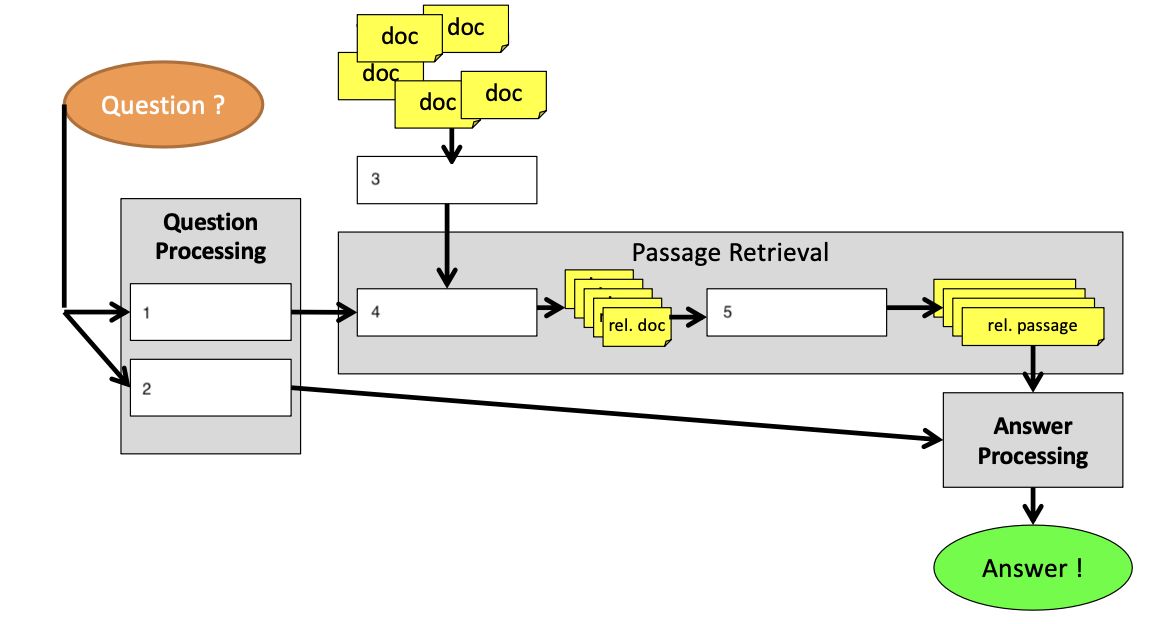
\includegraphics[width=.8\textwidth]{res/qa.png}
  \caption{Question Answering}\label{fig:qa}
\end{figure}

  Fill in the five white boxes in the image.

  \begin{solution}
    1. query formulation, 2. query classification, 3. indexing, 4. doc retrieval, 5. passage retrieval
  \end{solution}
\end{exercise}

\begin{exercise}{NLTK}
  Explain two parameters in NLTK that start with a "c".

  \begin{solution}
    \begin{itemize}
      \item \textbf{Chunking}: Identifies and groups words into syntactic chunks based on their POS tags.
      \item \textbf{Collocations}: Identifies words that frequently co-occur within a certain span.
      \item \textbf{Concordance}: Displays a word in context, showing its surrounding words within a specified window.
    \end{itemize}
  \end{solution}
\end{exercise}

\begin{exercise}{SVM}
  Explain Support Vector Machines when you have more than two classes.

  \begin{solution}
    \begin{itemize}
        \item \textbf{One-vs-One (OvO)}: Trains a classifier for every pair of classes. Final classification is determined by majority voting.
        \item \textbf{One-vs-All (OvA)}: Trains one classifier per class against all other classes. The highest-confidence prediction is chosen.
    \end{itemize}
  \end{solution}
\end{exercise}

\begin{exercise}{Feature differences}
  Explain the differences in features between classical ML and deep network-based ML.

  \begin{solution}
    \begin{itemize}
        \item \textbf{Classical ML} relies on manually engineered features (like tf-idf or n-grams) and requires domain expertise for feature extraction.
        \item \textbf{Deep networks} automatically learn hierarchical feature representations from raw data, capturing complex patterns and dependencies, but requiring large datasets for training.
    \end{itemize}
  \end{solution}
\end{exercise}

\begin{exercise}{Cohen's Kappa}
  \begin{table}
  \center
  \begin{tabular}{c|cc|c}
    Actual/Predicted& \textbf{+} & \textbf{-} & \\ \hline
    \textbf{+} & 10 & 5 & 15 \\
    \textbf{-} & 3 & 12 & 15 \\ \hline
    & 13 & 17 & \textbf{30} \\
  \end{tabular}
  \caption{Experimental resulsts}\label{tbl:results}
\end{table}
  Calculate Cohen's Kappa for Table \ref{tbl:results}.

  \begin{solution}
    Cohen's Kappa is calculated as $\kappa = \frac{P_o - P_e}{1 - P_e}$ and describes the observed agreement $P_o$ relative to the expected agreement $P_e$.
      \[ \kappa = \frac{.7333-.5}{1-.5} = \frac{0.2333}{0.5} = 0.4666 \]
  \end{solution}
\end{exercise}

\begin{exercise}{Evaluation metrics}
  \begin{table}
  \center
  \begin{tabular}{c|cc|c}
    Actual/Predicted& \textbf{+} & \textbf{-} & \\ \hline
    \textbf{+} & 10 & 5 & 15 \\
    \textbf{-} & 3 & 12 & 15 \\ \hline
    & 13 & 17 & \textbf{30} \\
  \end{tabular}
  \caption{Experimental resulsts}\label{tbl:results}
\end{table}
  Calculate Precision, Recall, and F1-Score for Table \ref{tbl:results}.

  \begin{solution}
    \begin{itemize}
        \item \textbf{Precision} $\frac{TP}{TP + FP} = \frac{10}{10+5} = .6666$
        \item \textbf{Recall}: $\frac{TP}{TP + FN} = \frac{10}{10+3} = .7692$
        \item \textbf{F1-Score}: $2 \times \frac{\text{Precision} \times \text{Recall}}{\text{Precision} + \text{Recall}} = 2 \times \frac{.6666 \times .7692}{.6666 + .7692} = .7142$
    \end{itemize}
  \end{solution}
\end{exercise}

\begin{exercise}{IR and classification}
  Where is classification used in Information Retrieval?

  \begin{solution}
    \begin{itemize}
        \item \textbf{Query classification}: Identify user intent (e.g., navigational vs. informational).
        \item \textbf{Document classification}: Categorize documents into predefined topics or genres.
        \item \textbf{Relevance classification}: Predict whether a document is relevant to a query.
    \end{itemize}
  \end{solution}
\end{exercise}

\begin{exercise}{Translate datasets}
  What are the pros and cons of translating datasets for NLP tasks? List 3 for each.

  \begin{solution}
    \begin{itemize}
        \item[+] Expands dataset availability to resource-scarce languages.
        \item[+] Enables cross-lingual NLP research.
        \item[+] Saves effort in recreating annotations.
        \item[-] Potential loss of annotation quality in translation.
        \item[-] Context or cultural relevance may not transfer.
        \item[-] Requires manual review to ensure correctness.
    \end{itemize}
  \end{solution}
\end{exercise}

\begin{exercise}{Web corpus}
  What are opportunities and challenges in using the web as a corpus?

  \begin{solution}
    \begin{itemize}
        \item[+] Large-scale, diverse data sources.
        \item[+] Includes up-to-date content.
        \item[+] Covers multiple languages and domains.
        \item[-] Noisy and unstructured data.
        \item[-] Contains duplicates and redundant information.
        \item[-] May include biased or low-quality content.
    \end{itemize}
  \end{solution}
\end{exercise}

\begin{exercise}{Pipeline}
  \begin{figure}
  \center
  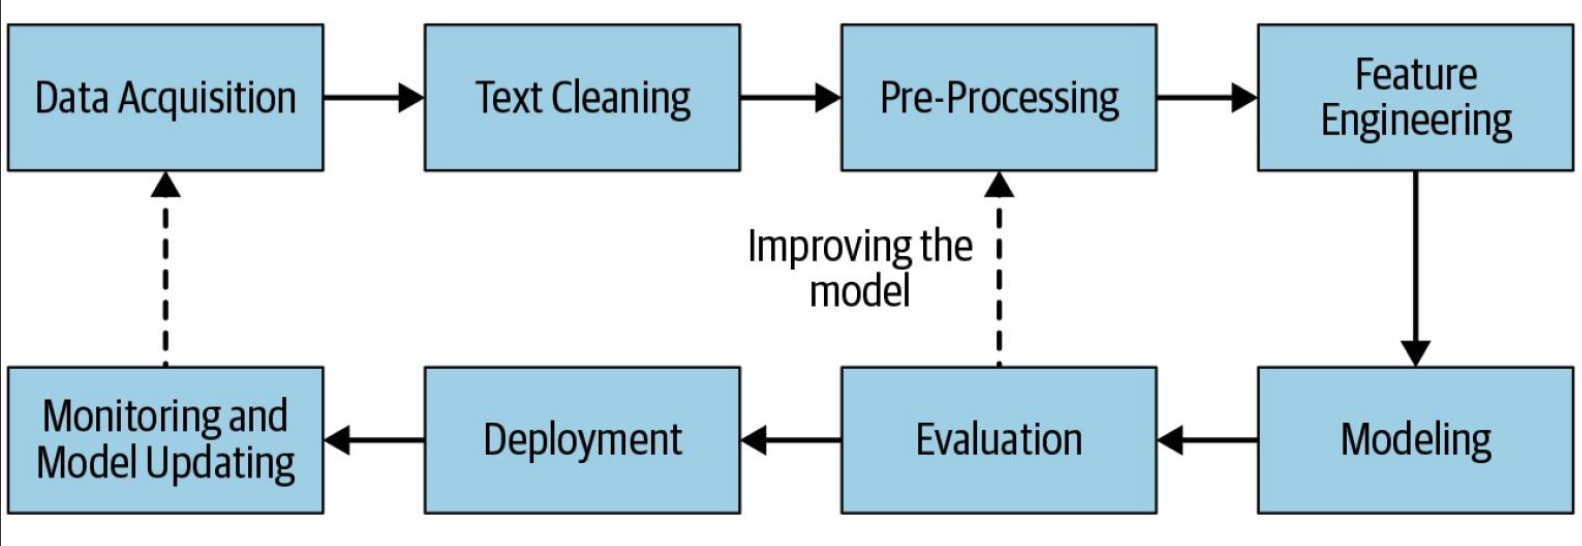
\includegraphics[width=.8\textwidth]{res/pipeline.png}
  \caption{NLP Pipeline}\label{fig:pipeline}
\end{figure}
  Assign three words to each stage of the given NLP pipeline in Figure \ref{fig:pipeline}.

  \begin{solution}
    \begin{itemize}
      \item \textbf{Data acquisition}: Crawling, scraping, downloading.
      \item \textbf{Text cleaning}: Tokenization, normalization, filtering.
      \item \textbf{Preprocessing}: Lemmatization, POS tagging, parsing.
      \item \textbf{Feature engineering}: TF-IDF, embeddings, n-grams.
      \item \textbf{Modeling}: Training, evaluation, and deployment.
      \item \textbf{Evaluation}: Metrics, analysis, feedback.
      \item \textbf{Deployment}: Integration, monitoring, maintenance.
      \item \textbf{Monitoring \& Model Updating}: Performance tracking, retraining, versioning.
    \end{itemize}
  \end{solution}
\end{exercise}

\begin{exercise}{MRR and accuracy}
  \begin{figure}
  \center
  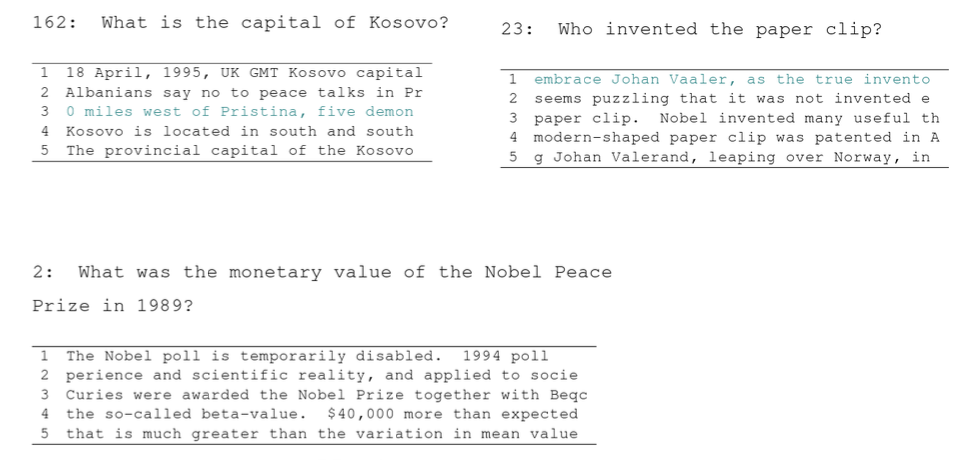
\includegraphics[width=.8\textwidth]{res/qa-answers.png}
  \caption{Question Answering}\label{fig:qa-answers}
\end{figure}
  Calculate MRR and Accuracy for the Question/Answering system in Figure \ref{fig:qa-answers}.

  \begin{solution}
    \begin{itemize}
        \item \textbf{Mean Reciprocal Rank} $MRR = \frac{1}{N} \sum_{i=1}^{N} \frac{1}{\text{rank}_i} = \frac{1}{3} (\frac{1}{3}+\frac{1}{1}+0 = .4444)$
        \item \textbf{Accuracy} $\frac{\text{Number of correct answers}}{\text{Total number of queries}} = \frac{2}{3} = .6666$
    \end{itemize}
  \end{solution}
\end{exercise}

\begin{exercise}{Language detection}
  Explain language detection and common approaches.

  \begin{solution}
    Language detection involves identifying the language of a given text.
    \begin{itemize}
        \item \textbf{N-gram analysis}: Compare character n-grams to language profiles.
        \item \textbf{Lexicon-based methods}: Match text to language-specific dictionaries.
        \item \textbf{Machine learning}: Train classifiers (e.g., SVM, neural networks) on labeled text.
        \item \textbf{Hybrid models}: Combine multiple techniques for higher accuracy.
    \end{itemize}
  \end{solution}
\end{exercise}

\begin{exercise}{Plagiarism detection}
  Explain three methods to detect plagiarism in text.

  \begin{solution}
    \begin{itemize}
        \item \textbf{String matching}: Use algorithms to find exact matches between documents.
        \item \textbf{Semantic similarity}: Apply embeddings to detect paraphrased or rephrased content.
        \item \textbf{Citation analysis}: Check for missing or incorrect citations.
        \item \textbf{Fingerprinting}: Generate hashes of text fragments and compare across sources.
    \end{itemize}
  \end{solution}
\end{exercise}

\begin{exercise}{Crowdsourcing}
  What are opportunities and challenges in using crowdsourcing for data annotation?

  \begin{solution}
    \begin{itemize}
        \item[+] Fast and scalable data annotation.
        \item[+] Access to diverse annotators.
        \item[+] Cost-effective compared to hiring experts.
        \item[-] Quality control is challenging.
        \item[-] May introduce noise or bias.
        \item[-] Difficult to ensure annotator expertise.
    \end{itemize}
  \end{solution}
\end{exercise}

\begin{exercise}{Recall improvement}
  Explain how to improve recall when using a search engine without changing the algorithm.

  \begin{solution}
    \begin{itemize}
        \item \textbf{Expanding queries}: Use synonyms, related terms, or stemming to match more results.
        \item \textbf{Reducing filters}: Remove restrictive criteria (e.g., date, location).
        \item \textbf{Boosting document recall}: Index more documents or reduce relevance thresholds.
    \end{itemize}
  \end{solution}
\end{exercise}

\begin{exercise}{Spell checker}
  How does a spell checker handle non-words?

  \begin{solution}
    \begin{itemize}
        \item \textbf{Dictionary lookup}: Identify words not in the dictionary.
        \item \textbf{Edit distance}: Suggest corrections based on similarity (e.g., Levenshtein distance).
        \item \textbf{Contextual models}: Use surrounding words to predict the intended word.
    \end{itemize}
  \end{solution}
\end{exercise}

\begin{exercise}{IR cycle}
  Explain the Information Retrieval cycle.

  \begin{solution}
    The IR cycle includes:
    \begin{itemize}
        \item \textbf{Indexing}: Process and store data for efficient retrieval.
        \item \textbf{Querying}: Users submit queries to search the index.
        \item \textbf{Retrieval}: Return ranked results based on relevance scores.
        \item \textbf{Evaluation}: Assess performance using metrics like precision and recall.
    \end{itemize}
  \end{solution}
\end{exercise}

\begin{exercise}{Vector space}
  Explain Vector Space in Information Retrieval.

  \begin{solution}
    \begin{itemize}
        \item \textbf{Terms}: Each dimension corresponds to a term in the vocabulary.
        \item \textbf{Weights}: TF-IDF scores are used as weights for each term.
        \item \textbf{Similarity}: Compute cosine similarity to rank documents by relevance to the query.
    \end{itemize}
  \end{solution}
\end{exercise}

\begin{exercise}{Sentiment analysis}
  Explain the difference between factual sentiment analysis and opinionated analysis.

  \begin{solution}
    \begin{itemize}
        \item \textbf{Factual sentiment analysis}: Focuses on extracting objective sentiment (e.g., product ratings).
        \item \textbf{Opinionated analysis}: Identifies subjective opinions (e.g., customer reviews).
        \item \textbf{Key difference}: Factual analysis is more structured and easier to evaluate, whereas opinionated analysis is subjective and context-dependent.
    \end{itemize}
  \end{solution}
\end{exercise}

\begin{exercise}{Sentiment analysis}
  Explain three areas where sentiment analysis is used.

  \begin{solution}
    \begin{itemize}
        \item \textbf{Customer feedback}: Analyze reviews for product improvements.
        \item \textbf{Social media monitoring}: Detect trends and public sentiment.
        \item \textbf{Political analysis}: Gauge public opinion on policies or events.
        \item \textbf{Market research}: Understand consumer preferences.
    \end{itemize}
  \end{solution}
\end{exercise}

\begin{exercise}{Teacher/Student}
  Explain the teacher/student signals approach in educational NLP and why it is better than pure audio content.

  \begin{solution}
    \begin{itemize}
        \item \textbf{Teacher signals}: Provide detailed instructions and explanations.
        \item \textbf{Student feedback}: Allows iterative learning and personalization.
        \item \textbf{Better than audio}: Interaction and adaptivity enhance understanding and retention compared to static audio content.
    \end{itemize}
  \end{solution}
\end{exercise}

\begin{exercise}{Representation and fusion}
  What are representation and fusion in multimodal NLP, and how do they differ?

  \begin{solution}
    \begin{itemize}
        \item \textbf{Representation}: Encodes data (e.g., text or images) into feature vectors.
        \item \textbf{Fusion}: Combines multiple data modalities (e.g., text and images) to improve performance.
        \item \textbf{Differences}: Representation focuses on individual modalities, whereas fusion integrates multiple modalities into a unified representation.
    \end{itemize}
  \end{solution}
\end{exercise}

\end{document}